\documentclass[12pt,a4paper, titlepage]{article}
% 页面边距调整
%\usepackage[top=1.5in, bottom=1.5in, left=1.5in, right=1.5in]{geometry}
\usepackage[top=1in, bottom=1in, left=1.25in, right=1.25in]{geometry}

\usepackage{epsfig}
\usepackage{subfig} %子图
\usepackage{fontspec}  %加這個就可以設定字體 
\usepackage{xeCJK}       %讓中英文字體分開設置 
%\usepackage{pinyin} %拼音
\usepackage{ruby}
\renewcommand{\rubysep}{-0.5ex}

%\usepackage{hyperref}
%\usepackage[hyphens]{url}
\usepackage[colorlinks]{hyperref}  %color support @ 
%{\color{red}显示的文字};green;blue;yellow。
%\usepackage[colorinlistoftodos]{todonotes}  %todo

\setlength{\parskip}{0.5\baselineskip} % 设定段间距
\linespread{1.2}                                      % 设定行距
\newcommand{\pozhehao}{\kern0.3ex\rule[0.8ex]{2em}{0.1ex}\kern0.3ex}
% 中文破折号,据说来自清华模板
\renewcommand{\contentsname}{目录} 
\renewcommand{\figurename}{图}

\setCJKmainfont{STFangsong}  %設定中文為系統上的字型,而英文不去更動,使用原TeX\字 
\XeTeXlinebreaklocale "zh"         %這兩行一定要加,中文才能自動換行 
\XeTeXlinebreakskip = 0pt plus 1pt  %這兩行一定要加,中文才能自動換行 

\author{@nixzhu \\ zhuhongxu@gmail.com}
\title{围棋急速入门}


\begin{document}
\setlength{\parindent}{2em}  
% 设定首行缩进为2em。注意此设置一定要在document环境之中,这可能与\setlength作用范围相关
\maketitle
\newpage

\tableofcontents	% 生成目录
\newpage
%=====================================================
\section{围棋的历史}
围棋,是一种策略性二人对战游戏\footnote{参见:\url{http://zh.wikipedia.org/zh-cn/\%E5\%9B\%B4\%E6\%A3\%8B}}。围棋起源于中国古代。推测起源时间为大约公元前6世纪\footnote{也就是说距今超过2500年了。},为“琴棋书画\footnote{对没有艺术天份的童鞋来说,学围棋以修身是唯一的选择。}”四艺之一。

围棋在公元7世纪传入日本。昭和\footnote{昭和是日本昭和天皇在位期间使用的年号,时间为1926年12月25日-1989年1月7日}时代,吴清源\footnote{真高手,参见:\url{http://zh.wikipedia.org/zh-cn/\%E5\%90\%B4\%E6\%B8\%85\%E6\%BA\%90}}和木谷实共同宣起了“新布局”的潮流,开始了现代围棋的时代。
1988年,曹薰铉在第一届应氏杯世界围棋锦标赛中夺冠,同样引发了韩国围棋的热潮。此后,大量世界性新闻棋战出现。在这些棋战中,李昌镐\footnote{高手,参见:\url{http://zh.wikipedia.org/zh-cn/\%E6\%9D\%8E\%E6\%98\%8C\%E9\%95\%90}}从众多棋手中脱颖而出,成为当时棋界第一人。2004年后,李昌镐的状态有所下滑,李世乭、古力等新锐势力开始对其发起冲击,国际棋战呈现中韩对抗,日本落后的局面。

目前围棋运动已遍布世界各地\footnote{大热西方的咏春拳也不错哦},唯中国、香港、台湾、日本、韩国最为兴盛;西方国家已渐热;东南亚正在发展中。

熟悉各种古代题材电视剧、电影的童鞋大概都见过古代的才子佳人、文人墨客或者高官政要下围棋。好像挺有品味的样子。我喜欢看《红楼梦》,对这部小说里面的下围棋的情节也有注意。可以发现,这些对弈者会在下棋的过程中表露他们自己的性格、意识等。有句话叫“棋品如人品”,大概有些道理。可能下围棋可以修身养性。

\section{围棋的规则}
按照我的理解,要看懂别人下棋,你至少要能回答三个问题:什么是吃?什么是死?什么是劫?

还有很多你从来没有听过的术语,但它们可以慢慢积累,不急。

我们先来看看棋盘,及其上面的棋子,看看它们可以提供什么信息给我们。

在图\ref{fig:qi}所示的棋盘上,有5堆棋子。先看棋盘的左下角,黑棋1有四条线链接到周围的4个空白交叉点,所以我们说,黑棋1有四口气;下面的白棋2在边上,由于边上没有延伸到棋盘外的线,即棋盘外没有交叉点,所以白棋2只有三口气;同理推之,黑棋3仅有两口气。从这里,你应该注意到棋子处于中腹、边或角的差别。这种差别会导致取舍的问题,就是做选择:是取地,还是取势。

那么图\ref{fig:qi}棋盘左上角的白棋4有几口气呢?按照定义,由白棋4延伸出去,只有右边有一个空白交叉点,其它三点被黑棋5、7、9占据,所以白棋4只有一口气。如果这个时候轮到黑棋下,而他又下在白棋4右边的空白点上,那么白棋4的气数就变为了零\footnote{这大概是成语“气数已尽”的来历},就是没气了死了,要被从棋盘上提走。那如果轮到白棋下,白棋该如何救回白棋4呢?很简单,也在相同的位置放置一颗白棋棋子,那么这个新的棋子就将白棋4、8链接在一起了,他们成为了一个“组合”,称为“一块棋”,相当于一个整体,共享它们所有的“气”,一起生,一起死。

\begin{figure}[htbp]   % 控制插图位置
	\setlength{\abovecaptionskip}{4pt}    
	\setlength{\belowcaptionskip}{4pt}
    %控制图形和上下文的距离
	\centering  % 使图形居中显示
	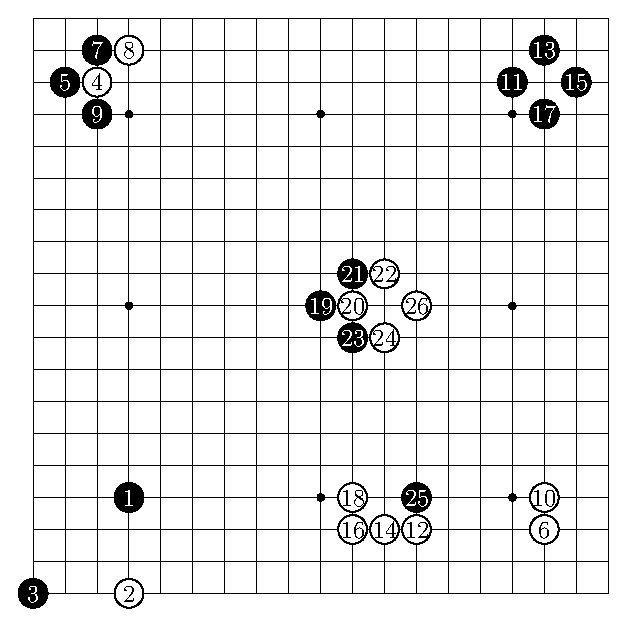
\includegraphics[width=0.5\textwidth]{fig/qi2.eps}
    %控制图形显示宽度为0.8\textwidth
	\caption{气}
	\label{fig:qi}
    %图形题目和交叉引用标签
\end{figure}

再来看看右下角的情况,白棋6、10是连接在一起的,所以它们可以共用“气”,数一下就知道,共有六口气。再数一下旁边的白棋18、16、14、12组成的棋块的气,有八口气,若没有黑棋25,则有九口气。

然后请将目光转向右上角,黑棋11、13、15、17没有链接在一起,但它们围住了一个“空”。这个空(也叫做气)是这四个子共用的。对于白棋来说,这个空就是死地,不能下去,因为处于这个位置的白棋无法向外面发出线条链接空白的交叉点,即找不到气。所以这个空白点对于白棋来说,就是“禁入点\footnote{禁止进入的点}”。

最后,请再将目光转到棋盘的中间,白棋20、22、24、26围住的空对于黑棋来说是“禁入点”吗?答案是“不是”。为什么?因为在围棋里有个原则,即,若本方的棋子将要落子的地方是个“禁入点”,但落子后能将对方的某些棋子提掉,则这个“禁入点”就不是真正的“禁入点”了。所以黑棋可以下,然后吃掉白棋20一子。

细心的童鞋就会发现,按照上面这样的规则,那白棋不是也可以提回来吗?之后黑棋也可以再提,那不是没完没了了吗?怎么办?

这个就是“劫”,后面会讲到,先有个概念就行了。

\subsection{什么是吃?}
围棋,顾名思义,是一种圈地的游戏。在$19 \cdot 19=361$的棋盘上,共有361个交叉点\footnote{边上和角上的特殊些,但也是交叉点。},也就是有361个“资源”。围棋的最终目的是想方设法使自己占有的资源超过对手。说简短些,就是使自己占有超过181\footnote{由于实战中执黑先行,终盘时黑方需要贴目,所以黑方大概需要超过185才能算胜,否则败}块“地”。

如何得“地”?原始人只有一个答案:争抢。必要时,要杀死对方的棋子\footnote{术语叫“吃”或“提子”}。前面介绍“气”的时候已经提到什么是吃,什么是没气,没有重复的必要。

\subsection{什么是活?}
还是从例子讲起吧?如图\ref{fig:huo}所示。
\begin{figure}[htbp]   % 控制插图位置
	\setlength{\abovecaptionskip}{4pt}    
	\setlength{\belowcaptionskip}{4pt}
    %控制图形和上下文的距离
	\centering  % 使图形居中显示
	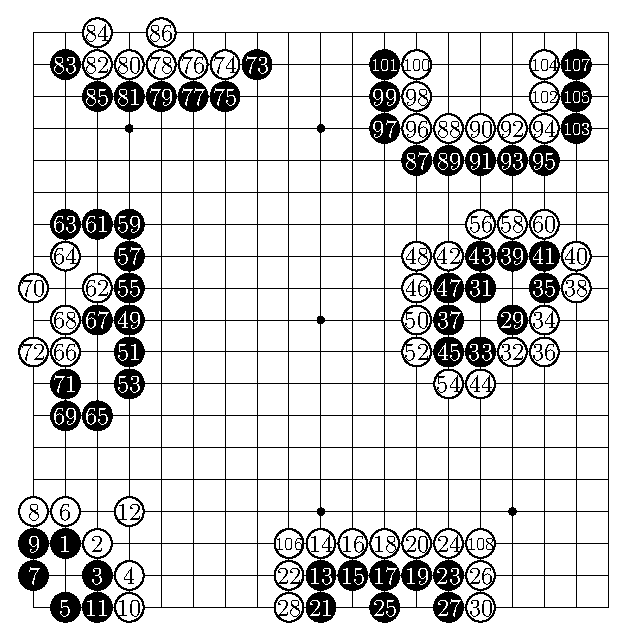
\includegraphics[width=0.5\textwidth]{fig/huo.eps}
    %控制图形显示宽度为0.8\textwidth
	\caption{活}
	\label{fig:huo}
    %图形题目和交叉引用标签
\end{figure}

先看图\ref{fig:huo}的左下角,6个黑子被围,而且黑棋是两块棋(并没有物理链接)。但是黑棋1、7、9组成的棋块和黑棋3、5、11组成的棋块共用两口气。若此时轮到白棋下,按照规则,黑棋围住的两个空对于白棋来说都是“禁入点”,而且没有例外情况(即白棋下在禁入点可以吃掉黑棋的情况)。所以这两块黑棋可以一直存留在棋盘上。对于这些黑棋的情况,有个定义,即,活棋。

同理,下边边上的黑棋虽然被围住,但依然有两口不能被同时堵住的气,我们说,黑棋有两个“眼”。所以要使一块棋在棋盘上生存下来,棋手必须保证他的这块棋至少能有两个眼,或者当前没有,但在将来有机会可以“做眼”。

说到“做眼”,请看看棋盘的左边,白棋被围住了(虽然不严密,但若继续走棋,就会完全封闭)。如果此时轮到白棋下,他该如何落子,以便做出两个眼来呢?可落子的地方并不多,稍微思考一下就会知道,应该下在64、62、57、61的中间。那如果轮到黑棋下,黑棋又该如何落子,以确保白棋不能做出两个眼来呢?答案是一样的。请读者思考一下。

棋盘右边的黑棋也被围住了,但是有两个眼,所以也是活棋。但是对比一下下边边上和角部的情况,可以知道,在中腹做活(即做出两个眼来)需要的子数较多,角部最少,边次之。

最后来看看上边的白棋,对于左边,黑棋如何下才能使白棋活不成?右边的呢?同样,若是白棋下,他又该如何做活呢?答案请读者思考。

\subsection{什么是劫?}
前面已经提到过劫了。劫,或者说“劫争”,是围棋上常见的一种激烈战斗的方式,其结果往往是你死我活。所以劫争非常重要。会制造劫、会打劫是一个棋手必备的技术。所谓“打劫”,就是两个棋手对一个劫的互相争夺。

\subsubsection{劫的定义}
\begin{figure}[htbp]   % 控制插图位置
	\setlength{\abovecaptionskip}{4pt}    
	\setlength{\belowcaptionskip}{4pt}
    %控制图形和上下文的距离
	\centering  % 使图形居中显示
	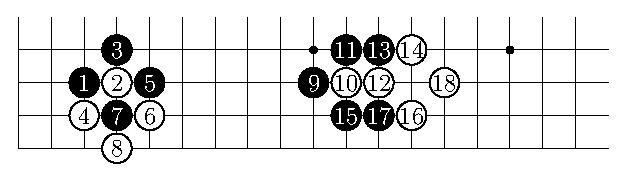
\includegraphics[width=0.5\textwidth]{fig/jie01.eps}
    %控制图形显示宽度为0.8\textwidth
	\caption{真劫与假劫}
	\label{fig:jie01}
    %图形题目和交叉引用标签
\end{figure}

图\ref{fig:jie01}显示的是劫。先看左边,黑7提掉了白2,这是规则允许的。但是白棋也可以重新在白2的位置落一个子,提掉黑7。黑棋也重新再来一次,…… 如果这个劫很重要,双方互不相让,就会没完没了。为了防止这种无法使棋局进行下去的局面。围棋的规则里就特别制定了关于“劫”的规则。

规定是这样的,黑7提掉白2之前,这一块当事棋\footnote{类比当事人}没有提子的前科。所以允许。但白棋想马上提回来,就不行了。因为劫已铸成,想打劫,就必须遵守规则。即,不能立即提回,必须间隔一手或多手棋。

那白棋想赢下这个劫争该怎么办呢?规则说,白棋,你可以在棋盘上除了白2的位置下一手棋,如果你逼迫到黑棋来应你\footnote{这种在打劫时在棋盘其他地方下棋并逼迫对方响应的手段叫做找劫材},对方若认为你刚刚下的这手棋威胁到他另外一些棋子的生存,而这些棋子的价值比刚才打劫的地方的价值要高,那么通常对方(黑棋)就会响应,转而防守白棋。

这时,距离黑7提吃白2已经过了两手棋(白一手,黑应一手)了。这个时候,如果白棋还想打劫,就可以在被提掉的白2位置落子,将黑7提去。

若黑棋心有不甘,想继续打劫。那么他也需要象白棋一样在棋盘的其他地方找个劫材,逼迫白棋接应。

当然,若黑棋找的劫材的价值小于当前打劫的价值,那么,白棋完全可以不应,而在黑7位置在落一子,消除打劫。

所以,一个劫是否需要打,能不能打赢,就要看你有没有劫材,有多少劫材啦。

再来看看图\ref{fig:jie01}右边的棋块。若轮到黑棋下,黑棋提吃白10、12两子后,白棋可以提回吗?答案是可以,因为这里并没有形成无限互提的局面。白棋只能提回一子而已。所以这个局面没有形成劫争。

\subsubsection{劫材}
前面讲了不少打劫的知识,问题的关键就是劫材。那么,什么是劫材?如何找劫材?如何判断一个劫材的价值?

劫材的定义是,在打劫(也叫劫争)的情况下,任何一方,为了打赢劫,而在棋盘的某一处下一子并逼迫对方应手的手段所利用的部位。这些劫材部位可能是对方棋子的缺陷处、或者“不应”就会损失很多的地方。

决定打劫前,因该先估计这个劫所含有的本位价值(及其延伸价值)。然后看看棋盘上有多少可利用的部位的价值大于此劫争的价值,也看看本方棋的缺陷会产生多少劫材,最后根据数目的对比决定是否需要打劫。如果你劫材不够,你是不可能打赢劫的。就算你表面上打赢了劫,也会在其他地方损失更多\footnote{所谓得不偿失}。

对于一个劫材的价值,需要读者自己思考,也需要经验的积累,当然也有一些书籍上介绍计算的方法。本教程作为围棋的急速入门教材,就不展开\footnote{事实上,我也很难展开}了。

\subsubsection{打劫的心得}
一个稍微会思考的人都会是理性的,围棋本身就是理性的,不乱下棋是一种重要的守则,就像在你的人生中不要乱作决定一样。打劫亦是如此。
\begin{enumerate}
\item 此劫对你来说,是否危险,即是否会因为劫争失败而输掉全盘。这称为“劫轻”或“劫重”。
\item 棋盘上是否存在更大的价值的地方可以争夺,这样就可以先不打劫。
\item 确定自己的劫材足够,或者不够但能在打劫的过程中制造一些以便劫材数超过对方,否者别打劫。
\end{enumerate}

\subsection{胜负计算}
新手学围棋,有个很大的困惑,就是如何计算胜负。

前面也说了,围棋是围地的游戏,终盘时,谁的地多,谁就赢。所以最简单的胜负计算方法是数自己棋子占据的交叉点数以及自己棋子围住的交叉点数之和。如果自己围住的部分有对方棋子的死子,要先将死子清除出棋盘。如果对方有争议,那就继续下到没有争议为止。

如果你是黑棋,且自己的点数之和超过一半(贴目的情况下大于一半,要大概185子),那么本方就胜利了,反之,败。

\section{可由经验积累的技术}
没有人天生就是高手,当然,天份是肯定有差别的。但所有人都必须由后天的习得来理解世界。围棋亦是如此。说一下我的经验吧。

在一开始,如果你对围棋很感兴趣,你会很用心的学习,但是与人对弈时,你总是输。然后你在学围棋的路上遇到困难了,你想放弃。可你心里还是很喜爱围棋,然后你重新来过。渐渐地,你就入门了,领会了围棋的奥妙,你真正喜欢上了围棋。

随着时间的推移,也许你又会降低自己的兴趣,原因可能是没有好的对手、棋力不再长进等。可是如果你坚持下来,过一段时间,你会发现,自己的棋力又长进了。你不会再怀疑自己的智商。

记得李昌镐说过,一个普通人学了围棋后可以很容易的达到5k的水平,但大多数人都止于此。少数有恒心的人会更进一步,达到业余初段的人不在少数。

所以学棋,贵在坚持。这也是人性中最宝贵的一种品质,让我们可以不断向前。

\subsection{术语}
看过电视围棋的朋友大概都了解,解说人员总是会从嘴了冒出些专业词汇,例如“断”、“粘”、“退”、“长”等。这些都是围棋术语,是为了更好的交流围棋而被广大棋手约定俗成的话语。它们都简洁有力,所以应该学习。但是不用专门学,遇到就学即可,反正也没多少个。

具体情况,请参见:\url{http://zh.wikipedia.org/zh/\%E5\%9B\%B4\%E6\%A3\%8B}

\subsection{定式}
所谓定式,就是黑白双方在角部\footnote{现代围棋对定式的定义不再局限于角部}的正确对应,也就是双方互不吃亏的最佳变化。即,局势两分,两方的收获和损失都差不多。

那为何要学定式?我的理解是,定式是快速熟悉围棋的好办法。学5、6个定式后就有这种感觉了。

首先,不要困惑。或者说:Don't Panic\footnote{参见《银河系漫游指南》里伟大的百科全书《银河系漫游指南》的封面}。你没有必要学习定式,定式是经验的总结。也就是说,经过足够长的时间,你可以“推导”出所有的定式。我就倾向于不学定式,我希望自己能感受到围棋的全部乐趣,包括“发现”定式的乐趣。

下面介绍两个比较有名的定式来凑一下字数。


\begin{figure}[htbp]   % 控制插图位置
	\setlength{\abovecaptionskip}{4pt}    
	\setlength{\belowcaptionskip}{4pt}
    %控制图形和上下文的距离
	\centering  % 使图形居中显示
	\subfloat[小目定式]{
		\label{fig:ds01}
		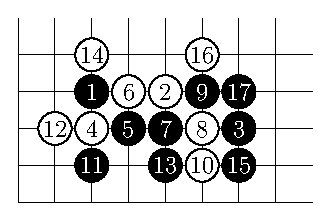
\includegraphics[width=0.2\textwidth]{fig/dingshi01.eps}
	}
	\hspace{15pt}
	\subfloat[星定式]{
		 \label{fig:ds02}
		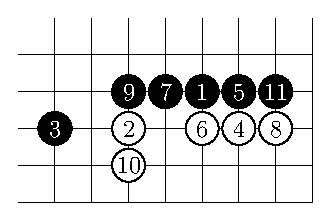
\includegraphics[width=0.2\textwidth]{fig/dingshi02.eps}
	}	
    %控制图形显示宽度为0.8\textwidth
	\caption{两个简单定式}
	\label{fig:dingshi}
    %图形题目和交叉引用标签
\end{figure}
先看图\ref{fig:dingshi}所示的两个定式。其中图\ref{fig:ds01}是一个小目定式,即黑1所在位置是小目。这个定式有一点点复杂,关键在于次序,即每一手棋之间的顺序。白14一定要先打吃,待黑15走后,白16再打吃。这样的局面是两分,白棋占优一点。所以如果你是黑棋,可能要避免选择这个变化。

图\ref{fig:ds02}是个简单的星定式,简单来说,白棋取得角地,黑棋取得外势。而且轮到白棋走,双方都可接受。

这两个例子都比较简单,但可窥一豹。定式有很多,而且也在不断的发展更新。所以要完整系统的学习定式,就需要买本书了。

\section{围棋进阶}
围棋的入门很容易,比如只有三条规则:吃、活、劫。但要熟悉围棋的本质“围地”还是需要些时间的。所以要让自己不断的练习学到的各种技术,最简单的办法就是找人对弈。现在网络这么方便,这一点很容易达到。网络围棋最重要的是礼仪,要有风度。

互联网是个巨大的学习宝库,各大视频分享网站上都有很多围棋的视频。例如youku上的围棋教学,王元8段的很有名。也有一些对局解说等。这些都是学习围棋的好材料。YouTube上的视频也不少,还有英文的,了解一下国外围棋的发展也不错哦。

再要进益。就看看吴清源先生的《黑布局》、《白布局》等,一些中盘战术的书,收官的书。因为一盘围棋从开局到结束可大致分为三个阶段:布局、中盘、收官。所以各个阶段的技术都要注意。

\subsection{进攻是最好的防守}
初学者大都不敢进攻对手,一切都小心翼翼,而且很多时候不知道该如何落子,心中没有任何概念。那么在这个时候,我的建议就是,放开手进攻对手的一块棋。在进攻中不断磨练自己的技术。最重要的是打开心结,寻找自信。

\subsection{防守是最好的进攻}
当你知道如何进攻别人之后,你就知道了别人会如何进攻你。对于自己的弱棋,一定要保护好,不给对方机会。如果你给对手留下太多缺陷,你就会一直被动,疲于防守。结果就可想而知了。

\subsection{掌握平衡}
围棋里有个术语叫“过分”。凡事都不能过界,围棋也一样。如果你太过深入敌后以便侵消对手实地,就会遭到对手的猛烈反击,最坏的结果是全军覆没。当然,若对手实力不济,就可以胜利了。所以对弈时要适当的评估对手,特别是你不熟悉的对手(网络围棋通常就是这种情况)。掌握他们的喜好,分析他们的棋路,以便合理对应。

\subsection{争先}
在平衡的基础上,要尽量争先,先手优势是非常重要的。吴清源先生说过,高手下棋都会费尽心思去取得一个先手,以便能掌控或引导接下来的对局,将局势导向有利自己的一面。

围棋的模式是从活跃的状态逐渐变为固定的状态。每下一步都不能回头,所以一定要三思而后行。思考是学围棋必须要懂的。你要考虑自己的弱点、优点,对方的弱点、优点,双方的实地对比、外势对比等。心中要有个概念,不要到局终了还不知道是自己是赢是输。

\section{结语}
我尽量将围棋的规则讲的简易些,能使爱好围棋的初学者快速入门,顺便给他们一些鼓励和安慰。

我本身也不是围棋高手,只算个刚刚入了门的爱好者罢。前面很多都是自己的一面之词,不可全信。本文的写作动力是想看看我编写的sgf2asy\footnote{一个将SGF格式的围棋棋谱转为Asymptote矢量脚本的Python脚本 \url{https://github.com/nixzhu/sgf2asy}}程序的工作情况,顺便总结一下自己的围棋心得。本文的参考文献主要是维基百科上的围棋条目,以及大竹英雄写的《围棋初级指导》。

希望看官指出错误,给些意见或建议。有机会我再丰富本文。

Twitter:\url{http://twitter.com/nixzhu}
Email:\href{mailto:zhuhongxu@gmail.com}{zhuhongxu@gmail.com}

\end{document}
